\chapter{Theoretical Background}
This chapter introduces some background knowledge related to
terrain rendering and geographical information systems (GIS).

\section{Basics of Terrain Rendering}
\subsection{Terrain Data Representations}
One of the central aspects of terrain rendering 
is the underlying data representing the terrain.
The following subsections introduce the two most important 
ways of representing terrain data and
lists some of their strengths and weaknesses.

\subsubsection{Heightmaps}
The surface of a terrain can be represented
with a regular grid of height values.
When storing such height values in an image, the resulting 
image is called a \textit{heightmap}. Each pixel 
in the heightmap contains a color value, which corresponds 
to the height of the terrain at that particular image coordinate. 
Normally, low color values correspond to low elevation 
and high color values to high elevation. Figure \ref{fig:results-heightmap}
shows an example of a 16-bit greyscale heightmap of a large part of Switzerland
and its neighboring countries.

\begin{figure}[H]
  \centering
  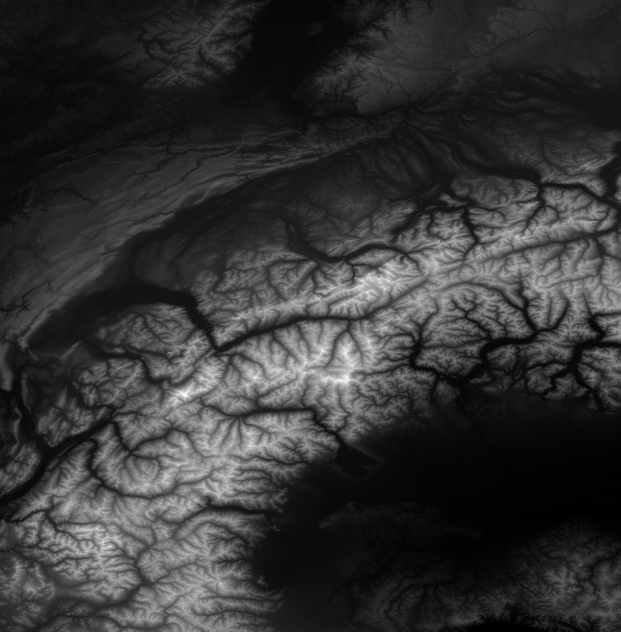
\includegraphics[width=0.7\textwidth]{results-heightmap}
  \caption{The $13922 \times 14140$ 16-bit greyscale heightmap of a large part of Switzerland and neighboring countries (retrieved from OpenTopography \cite{srtm2013}). In this figure, the gray values were converted from 0,\dots,65535 to 0,\dots,255 in order to make the heights more visible.}\label{fig:results-heightmap}
\end{figure}

The main advantage of heightmaps is that height data 
can be stored and retrieved very efficiently,
requiring only the actual height value to be stored per position
instead of the entire $(x,y,z)$ coordinate. 
Another advantage of heightmaps is that they can be 
used as textures on the GPU, which has been basis for many
modern GPU-based terrain LOD algorithms (see subsection ``Categorization of Terrain LOD Algorithms'').

The main weakness of heightmaps is that they are limited to 
a single height value per $(x,z)$ coordinate. Special 
terrain features such as cliffs, overhangs or caves 
cannot be modelled only with heightmaps and require 
special handling \cite{lodfor3dgraphics}.

Heightmaps are used extensively in game engines.
The Unity game engine for example stores heightmaps as 16-bit-per-color 
grayscale RAW images, allowing for $2^{16} = 65536$ different height values.

\subsubsection{Triangulated Irregular Networks}
An alternative representation of a terrain's surface is the \textit{triangulated irregular network (TIN)}.
The TIN is a data structure that consists of 3-dimensional points
which make up a triangulated mesh.
This means that when viewed from above (i.e. from the $(x,z)$ plane), 
the distance between any two neighboring points can be irregular,
which is not the case with heightmaps. TINs 
are often generated using heightmaps themselves for 
height information.

Figure \ref{fig:tin-example} shows two examples of TINs;
a TIN with a highly variable surface and a TIN with a 
less variable surface.

\begin{figure}[H]
  \centering
  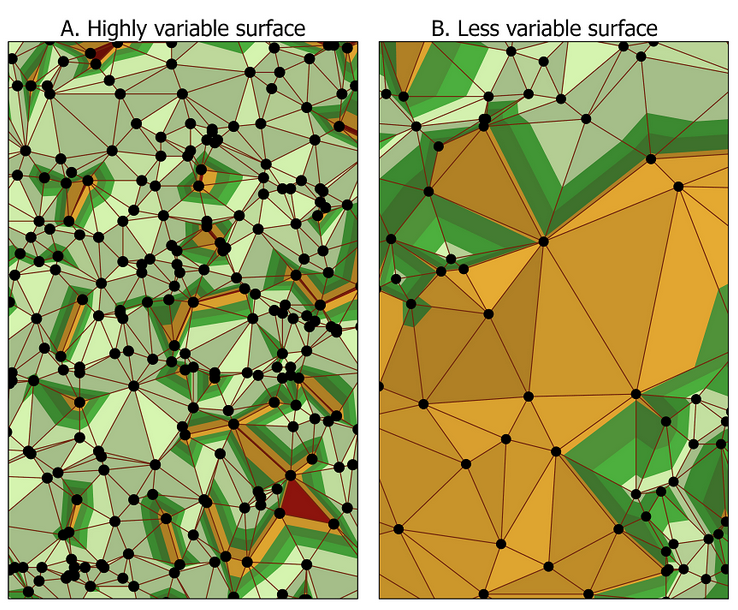
\includegraphics[width=0.75\textwidth]{tin-example.png}
  \caption{Two examples of TINs: a TIN with a highly variable surface (A) and a TIN with a less variable surface (B) (image source: \cite{tinimage}).}\label{fig:tin-example}
\end{figure}

The main advantage of TINs is that unnecessary information 
in the terrain can be eliminated. For instance, flat areas with little variation 
in height can be represented with few vertices. 
Another advantage is that special terrain features, 
such as cliffs or overhangs, can be modelled easily, 
since each point is a three-dimensional vertex.

A disadvantage of TINs is that they 
are more expensive to compute and prepare, especially 
when taking LOD into account.
Another disadvantage of TINs is that 
they now require the full $(x,y,z)$ vertices 
to be stored per point in the TIN, whereas with 
heightmaps, only a single color value per height is required.

\subsection{Categorization of Terrain LOD Approaches}
The following categorization of terrain LOD algorithms 
is partially based on chapter ``Massive-Terrain Rendering'' from the book \textit{3D Engine Design for Virtual Globes} by Ring and Cozzi \cite[p.~365]{3denginedesignforvirtualglobes}. 

\paragraph{Discrete LOD} \textit{Discrete LOD} algorithms 
usually work on discrete blocks or patches of terrain. 
These blocks are usually organized into multiple LOD resolutions.
Some examples of discrete LOD algorithms include GeoMipMapping \cite{geomipmapping}
and Geometry Clipmaps \cite{geomclipmaps}.

\paragraph{Continuous LOD} \textit{Continuous LOD} algorithms
usually operate on single triangles and vertices and dynamically 
modify the mesh at runtime. Continuous LOD algorithms are not
widely used today, since modifying the mesh on 
a frame-to-frame basis at runtime is less performant 
than the alternative of simply storing terrain blocks 
on the GPU in advance\cite[p.~368]{3denginedesignforvirtualglobes}. For this reason, this thesis 
will not continue discussing continuous LOD algorithms.
Some examples of continuous LOD algorithms include 
\textit{ROAM} \cite{roam} and \textit{SOAR} \cite{soar}.

\paragraph{Hierarchical LOD} \textit{Hierarchical LOD} algorithms
are similar to discrete LOD algorithms in the sense 
that they organize the terrain in discrete blocks.
The main difference is that hierarchical LOD algorithms organize the blocks 
hierarchically so that the data further up
in the hierarchy represents larger areas at lower resolutions
and the data lower in the hierarchy represents more detailed areas 
at higher resolutions. The actual mesh can be either grid-based, as in 
GeoMipMapping or Geometry Clipmaps, but it can also be 
based on TINs. The most well-known example of a hierarchical LOD algorithm 
is Chunked LOD \cite{chunkedlod}.

A small selection of terrain LOD algorithms relevant for this thesis will 
be summarized in chapter ``Previous Work''.

\subsection{Potential Problems during Rendering}
\subsubsection{Low Framerates}
As already indicated in the introduction chapter,
the most prevailing problem during terrain rendering 
and the main motivation behind terrain LOD algorithms
is a bad rendering performance due to the massive number of
rendered triangles. 
Systems that render terrains must be able to do so 
with decent framerates of at least 60 frames per second.
A low framerate destroys immersion of the user and 
puts a major strain on the GPU.

\subsubsection{Cracks}
When rendering terrains with LOD, a common scenario is 
that a terrain region close to the camera with more detail
borders another region of terrain further away with less detail.
Without any special treatment, this scenario can cause a visual disturbance in the terrain,
a so-called \textit{crack}. Cracks occur when certain vertices of the higher resolution terrain mesh 
lie below the edge of the lower resolution terrain mesh, as illustrated in figure \ref{fig:crack-example}.

\begin{figure}[H]
  \centering
  \subfloat[\centering]{{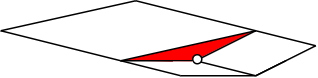
\includegraphics[width=0.4\textwidth]{crack-illustration.png} }}
  \qquad
  \subfloat[\centering]{{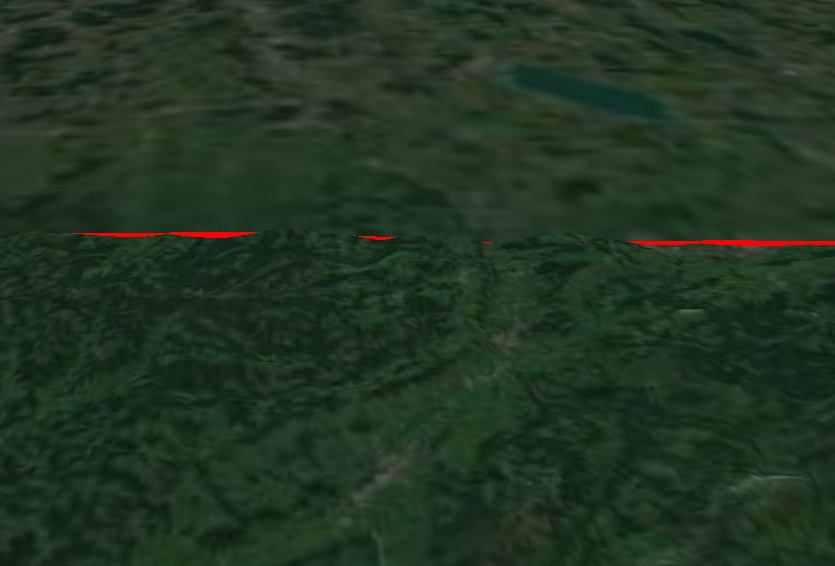
\includegraphics[width=0.4\textwidth]{crack-example.png} }}%
  \caption{An illustration (a) and a render (b) of a crack occuring between two terrain sections with different LOD levels. The background was colored red in both subfigures for visibility.}\label{fig:crack-example}
\end{figure}

Cracks can be avoided in a number of ways. 
One approach is to organize the terrain meshes in such a 
way that such crack-causing vertices can never occur in the first place.
This approach is used in numerous terrain LOD algorithms, 
such as GeoMipMapping \cite{geomipmapping}, ROAM \cite{roam} and others.
The main advantage of this approach is that it ensures
a continuous terrain mesh. The disadvantage is 
that it requires potentially more complex mesh processing and 
triangulation times.

Another approach is to render \textit{skirts}
around the terrain meshes, which drape downwards 
and repeat the overlay texture at the border. 
This approach is used in various 
terrain LOD algorithms as well, such as 
Chunked LOD \cite{chunkedlod}, Geometry Clipmaps \cite{geomclipmaps}
and others. The main advantage of skirts is that they 
are very simple to implement.
The main disadvantage is that they require more triangles 
to be rendered and are thus slightly more expensive to render. Another disadvantage
is that skirts are only hiding 
the cracks instead of completely removing them.

\subsubsection{Popping}
\textit{Popping} is a visual artifact 
that occurs when the camera is flying towards 
a lower resolution terrain section and 
the sudden change in LOD level of the terrain section 
to a higher LOD level causes a visual popping-in of more detail
into the screen.

Popping can be avoided in a number of ways.
The first solution is \textit{geomorphing} \cite{wikipediapopping}.
With geomorphing, the vertices of the higher and 
lower resolution terrain meshes are interpolated,
such that a smooth transition occurs during when 
flying closer to the target terrain mesh.
Another solution is \textit{LOD blending} \cite{wikipediapopping},
which simply blends the alpha or transparency channel of 
both the high and the low resolution mesh of the same 
terrain section, at the cost of having to render both meshes 
at the same time.

\subsubsection{Precision Issues}
A set of common issues for particularly large 
and detailed terrains are \textit{precision issues}.
Most graphics APIs today rely on 32-bit floating point 
numbers by default. When using 32-bit floating point 
numbers for transforming vertices with very large coordinates, this can lead to \textit{jittering},
i.e. vertices shaking on the screen due to roundoff errors.
The depth buffer also suffers from limited precision (24 bits in OpenGL by default), which may lead to 
\textit{depth buffer fighting}, where objects on the screen 
which are close to each other flicker repeatedly due to roundoff errors in the depth buffer.

The reference book \textit{3D Engine Design for Virtual Globes} by Cozzi and Ring 
lists a few common solutions for handling precision issues 
for both vertex transformation imprecision and depth buffer imprecision.
Vertex transformation imprecision artifacts can be avoided by 
using OpenGL's double precision support (when supported), 
\textit{relative-to-center rendering} \cite[p.~164]{3denginedesignforvirtualglobes}, 
\textit{relative-to-eye rendering} \cite[p.~169]{3denginedesignforvirtualglobes}, 
or when applicable, scaling down coordinates.
Depth buffer imprecision artifacts can be avoided 
with \textit{complementary depth buffering} \cite[p.~189]{3denginedesignforvirtualglobes},
\textit{logarithmic depth buffering} \cite[p.~191]{3denginedesignforvirtualglobes}
and \textit{rendering using multiple view-frustums} \cite[p.~194]{3denginedesignforvirtualglobes}.

\section{Digital Cartography}
This section introduces a selection of concepts from geographical information systems 
which will later be important for accurately rendering the Earth in StreamingATLOD.

\subsection{Ellipsoids}
The Earth, despite vocal objections by many throughout the course of history, is not flat.
Contrary to popular belief, the Earth is not entirely spherical either,
but \textit{ellipsoidal}. This means that the 
radius of the Earth is not the same in the $(x,y,z)$ directions. 
An ellipsoid is defined with three radii $\mathbf{r}_{ellipsoid} = (r_x,r_y,r_c)$ 
and each point $(x,y,z)$ on the surface of the ellipsoid must satisfy the following equation \cite[p.~17]{3denginedesignforvirtualglobes}:
\begin{align*}
\frac{x^2}{r_x^2} + \frac{y^2}{r_y^2} + \frac{z^2}{r_z^2} = 1.  
\end{align*}

The choice of $\mathbf{r}_{ellipsoid}$ is an important aspect for rendering globes.
The \textit{WGS84 ellipsoid} is defined with the radii $(6378137, 6378137, 6356752.314245)$ and 
is commonly used in other virtual globe systems \cite[p.~19]{3denginedesignforvirtualglobes}.
As will be explained later in chapter ``StreamingATLOD'', we use smaller radii for StreamingATLOD in order to avoid 
precision issues during rendering.

\subsection{The WGS84 Coordinate System}
The \textit{World Geodetic System 84 (WGS84)} coordinate system
(EPSG:4326) is a geographic reference system that
was introduced in 1984. 

A geodetic coordinate in WGS84 consists of three components:
\begin{itemize}
  \item The \textit{longitude} is measured in degrees
  in a range from $-180^\circ$ to $180^\circ$ and goes from west to east.
  The longitude at $0^\circ$ is called the \textit{Prime Meridian}
  and lies roughly where Greenwich, UK is.
  \item The \textit{latitude} is measured in degrees as well 
  in a range from $-90^\circ$ to $90^\circ$ and goes from south to north.
  The latitude at $0^\circ$ is called the \textit{Equator} 
  and lies in the middle between the North and South Pole.
\end{itemize}

In order to render globes, geodetic coordinates must be transformed into 
cartesian coordinates and vice-versa.
The various conversion formulas and their derivations can be found in 
chapter ``Math Foundations''
in the book \textit{3D Engine Design for Globe Rendering} 
by Cozzi and Ring \cite[p.~13]{3denginedesignforvirtualglobes}.

\subsection{The Web Mercator Projection}
Even though the Earth is not flat, for some purposes it is easier 
to treat the Earth as a flat plane, for example when rendering 
2D maps.
A \textit{map projection} projects geodetic coordinates from a spherical or ellipsoidal model onto a flat plane.
The main map projection used in this thesis is the \textit{Web Mercator projection}.
It distorts the scale at the poles, making the North and South Poles
famously appear larger than they really are, as shown in figure \ref{fig:tissot-indicatrix}.

\begin{figure}[H]
  \centering  
  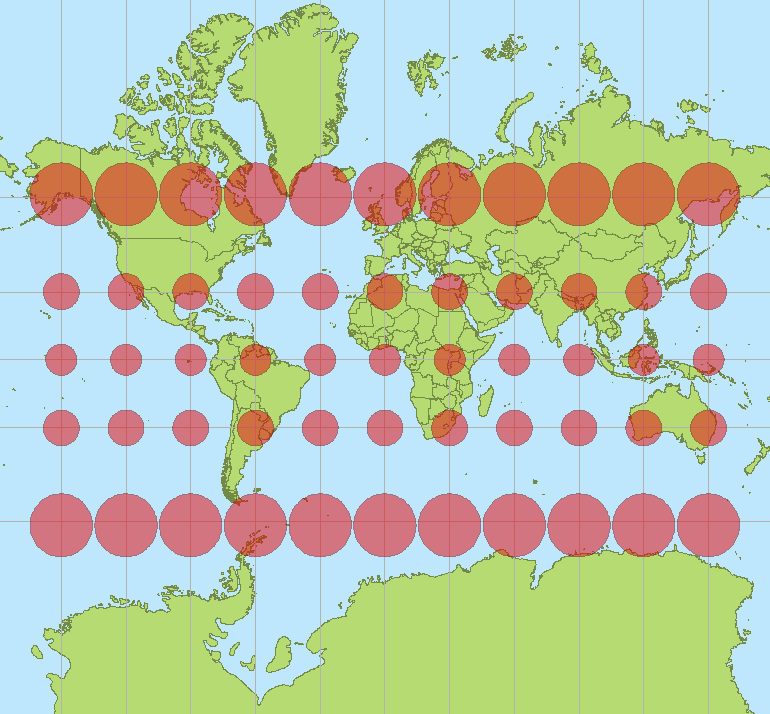
\includegraphics[width=0.4\textwidth]{tissot-indicatrix.png}
  \caption{Tissot's indicatrix showcasing the distortion in the Mercator projection (image source: \cite{wikipediatissotindicatrix}).}\label{fig:tissot-indicatrix}
\end{figure}

The Web Mercator projection is based on the 
regular \textit{Mercator projection} and was introduced and popularized by Google Maps. 
The main difference between the Mercator and the Web Mercator projection lies in 
the fact that the Web Mercator projection cuts off 
the latitude at $\pm 85.051129^{\circ}$
in order to make images fit into a square \cite{wikipediawebmerc}.

The formula for the Web Mercator projection yields the projected $(x,y)$ coordinates given a longitude and a latitude \cite{webmerc}:
\begin{align*}
  x &= lon,\\
  y &= \ln \Big(\tan \Big( \frac{\pi}{4} + \frac{lat}{2}\Big)\Big).
\end{align*}

The \textit{Inverse Web Mercator projection} yields the longitude and latitude 
given projected $(x,y)$ coordinates \cite{webmerc}:
\begin{align*}
  lon &= x,\\
  lat &= \frac{\pi}{2} - 2 \arctan (\exp(-y)).
\end{align*}

\subsection{Map Tiling}
Managing and rendering maps and geographic data requires that they are split up into manageable segments
with multiple resolutions. This process is called \textit{map tiling} and is essentially 
the concept of LOD applied to geographic data. It is usually applied to 
images, such as cartographic or satellite images, or chunks of 
geospatial data inside a bounding rectangle. A \textit{tile} refers to 
a single image or chunk at a particular position and a \textit{zoom level}.
The term \textit{zoom level} is equivalent to the term \textit{LOD level} in LOD rendering.

There exist numerous standards for map tiling, such as \textit{XYZ tiles} (also called \textit{ZXY tiles}) by Google Maps,
the \textit{Tile Map Service (TMS)} by OpenLayers, the \textit{Web Map Tile Service (WMTS)}
by the Open Geospatial Consortium (OGC), \textit{Quadkeys} by Bing Maps, and more.
All those standards organize the tiles hierarchically, such that each 
tile has four child tiles.
Figure \ref{fig:tiling-schemes} shows a comparison of tile indexing methods
for different tiling standards.

\begin{figure}[H]
  \centering  
  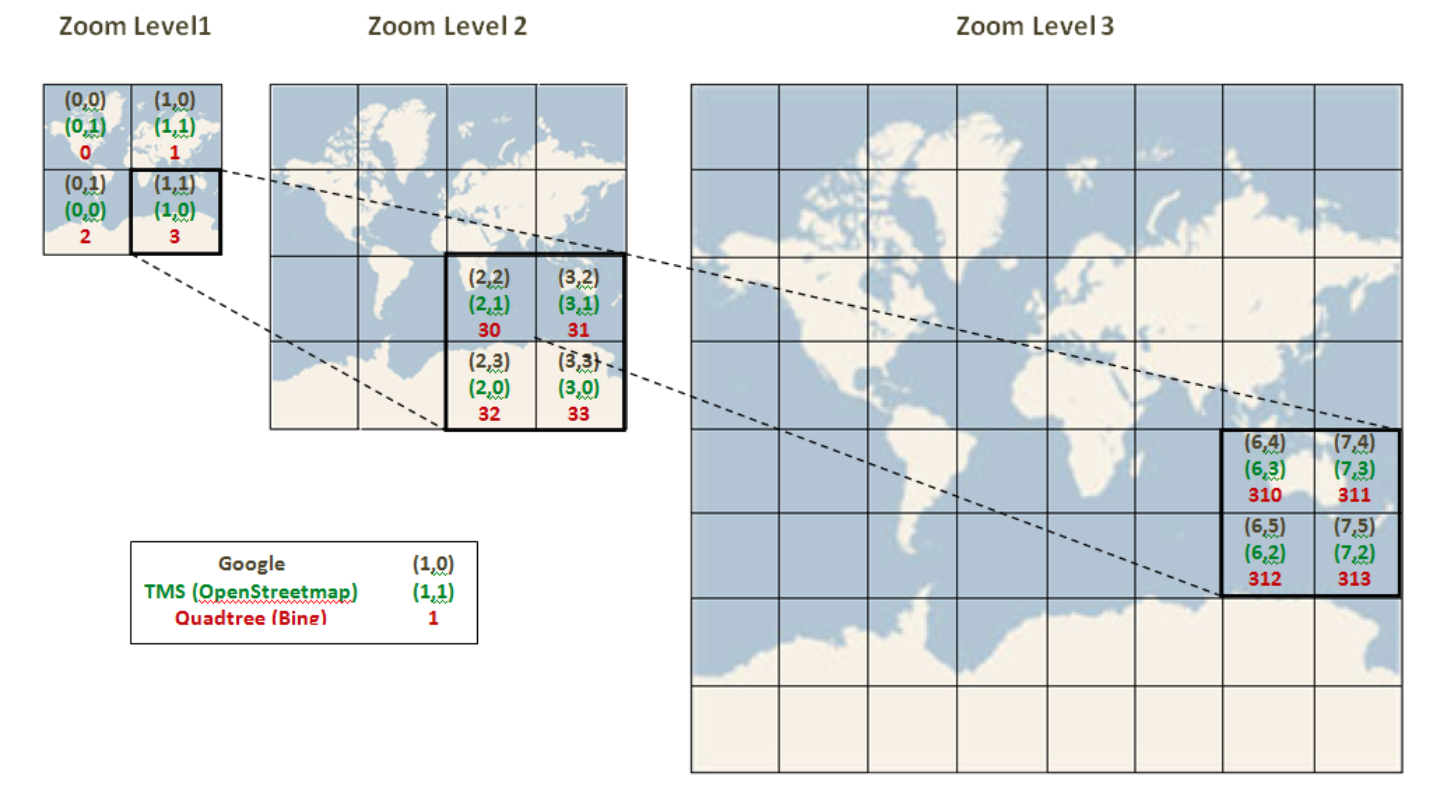
\includegraphics[width=1\textwidth]{tiling-schemes.png}
  \caption{A comparison of tile indexing methods for Google Maps, Bing Maps and TMS (image source: \cite{tileimage}).}\label{fig:tiling-schemes}
\end{figure}

For this thesis, the most relevant map tiling scheme is the \textit{XYZ tiling scheme}. 
Each of the four child tiles represents a fourth of the parent tile's area, but at twice the resolution.
Usually, every tile has the same pixel resolution, regardless of the current zoom level.
Each tile has an $x$, $y$, and $z$-coordinate associated with it. 
The full triple is called the \textit{tile key} and is denoted $tk = (tk_x, tk_ y, tk_z)$ in this report. 
The $x$ and $y$ coordinates represent the position of the tile 
horizontally and vertically respectively, and the $z$-coordinate 
denotes the zoom level of the tile. Each tile can be 
uniquely identified with a single tile key.
The $(x,y)$ coordinates 
begin from the top-left corner and go to the bottom-right corner and the $z$ coordinate 
starts from 0 (lowest resolution) and grows up to a maximum zoom level.
The four child tiles of a given tile $(tk_x,tk_y,tk_z)$ are computed as follows: 
\begin{itemize}
  \item Top-left child tile: $(2 \times tk_x, 2 \times tk_y, tk_z + 1)$
  \item Top-right child tile: $(2 \times tk_x + 1, 2 \times tk_y, tk_z + 1)$
  \item Bottom-left child tile: $(2 \times tk_x, 2 \times tk_y + 1, tk_z + 1)$
  \item Bottom-right child tile: $(2 \times tk_x + 1, 2 \times tk_y + 1, tk_z + 1)$
\end{itemize}

As a basic example, consider the scenario of having XYZ tiles of satellite imagery of the Earth.
The zoom level 0 contains a single tile, the root tile, which has the XYZ tile key of $(0,0,0)$ 
and contains the entire Earth at the lowest resolution. 
The four child tiles at zoom level 1 are the top-left tile $(0,0,1)$, the top-right tile $(1,0,1)$,
the bottom-left tile $(0,1,1)$ and the bottom-right tile $(1,1,1)$.

XYZ tiles are ususally served on web servers 
with an URL scheme of \\ \texttt{http://www.example.com/z/x/y.ext},
where \texttt{z} corresponds to the zoom level, 
\texttt{x} and \texttt{y} to the tile coordinates
and \texttt{.ext} to the file extension, such as \texttt{.png} or \texttt{.jpg} \cite{wikipediatiledwebmaps}.